%  LaTeX support: latex@mdpi.com 
%  In case you need support, please attach all files that are necessary for compiling as well as the log file, and specify the details of your LaTeX setup (which operating system and LaTeX version / tools you are using).

%=================================================================
\documentclass[sensors,article,submit,moreauthors,pdftex]{Definitions/mdpi} 
\firstpage{1} 
\makeatletter 
\setcounter{page}{\@firstpage} 
\makeatother
\pubvolume{xx}
\issuenum{1}
\articlenumber{5}
\pubyear{2019}
\copyrightyear{2019}
%\externaleditor{Academic Editor: name}
\history{Received: date; Accepted: date; Published: date}
%\updates{yes} % If there is an update available, un-comment this line

%% MDPI internal command: uncomment if new journal that already uses continuous page numbers 
%\continuouspages{yes}
\usepackage{subfigure}
\usepackage{balance}
\usepackage{tabularx}

%-------------------------------------------------
\newcommand{\TG}[1]{\color{red}\textbf{From Dr.Glatard}: #1\color{black}}
\newcommand{\TGB}[1]{\color{blue}\textbf{From Behzad}: #1\color{black}}
\newcommand{\TGS}[1]{\color{green}\textbf{From Dr.Shihab}: #1\color{black}}
\newcommand{\TGO}[1]{\color{green}\textbf{From Omid}: #1\color{black}}

%------------------------------------------------------------------
% The following line should be uncommented if the LaTeX file is uploaded to arXiv.org
%\pdfoutput=1

%=================================================================
% Add packages and commands here. The following packages are loaded in our class file: fontenc, calc, indentfirst, fancyhdr, graphicx, lastpage, ifthen, lineno, float, amsmath, setspace, enumitem, mathpazo, booktabs, titlesec, etoolbox, amsthm, hyphenat, natbib, hyperref, footmisc, geometry, caption, url, mdframed, tabto, soul, multirow, microtype, tikz

%=================================================================
%% Please use the following mathematics environments: Theorem, Lemma, Corollary, Proposition, Characterization, Property, Problem, Example, ExamplesandDefinitions, Hypothesis, Remark, Definition, Notation, Assumption
%% For proofs, please use the proof environment (the amsthm package is loaded by the MDPI class).

%=================================================================
% Full title of the paper (Capitalized)
\Title{A quantitative comparison of Overlapping and Non-overlapping sliding windows for human activity recognition using wearable sensors}

% Author Orchid ID: enter ID or remove command
\newcommand{\orcidauthorA}{0000-0000-000-000X} % Add \orcidA{} behind the author's name
%\newcommand{\orcidauthorB}{0000-0000-000-000X} % Add \orcidB{} behind the author's name

% Authors, for the paper (add full first names)
\Author{Akbar Dehghani$^1$, Omid Sarbishei$^2$, Tristan Glatard$^1$, Emad Shihab$^1$}

% Authors, for metadata in PDF
\AuthorNames{Akbar Dehghani, Omid Sarbishei, Tristan Glatard, Emad Shihab}

% Affiliations / Addresses (Add [1] after \address if there is only one affiliation.)
\address{%
$^{1}$ \quad Department of Computer Science and Software Engineering, Concordia University, Montreal, QC, Canada \\
$^{2}$ \quad Research and Development Department, Motsai Research, Saint Bruno, QC, Canada}

% Contact information of the corresponding author
\corres{Correspondence: eshihab@encs.concordia.ca}

% Current address and/or shared authorship
%\firstnote{Current address: Affiliation 3} 
%\secondnote{These authors contributed equally to this work.}
% The commands \thirdnote{} till \eighthnote{} are available for further notes

%\simplesumm{} % Simple summary

%\conference{} % An extended version of a conference paper

% Abstract (Do not insert blank lines, i.e. \\) 
\abstract{The sliding window technique is widely used to segment sensor signals for Activity Recognition. In this technique, the sensor signals are partitioned into fix-sized time windows which can be of two types: (1) non-overlapping windows, in which time windows do not intersect, and (2) overlapping windows, in which they do. There is a generalized idea about the positive impact of using overlapping sliding on the performance of recognizer systems in Human Activity Recognition. 
In this paper, we analyze the impact of overlapping sliding windows on the performance of Human Activity Recognition systems with different evaluation techniques, namely subject-dependent cross validation and subject-independent cross validation. Our results show that the overlapping windowing improvements reported in the literature seems to be associated with the underlying problems of subject-dependent cross validation. Furthermore, we do not observe any performance gain from the use of such technique in conjunction with subject-independent cross validation. We conclude that when using subject-independent cross validation,
non-overlapping sliding windows reach the same performance as sliding windows. This result has significant implications on resource usage, a big concern in embedded systems.}

% Keywords
\keyword{Activity recognition; Wearable sensors; Supervised classification}

%%%%%%%%%%%%%%%%%%%%%%%%%%%%%%%%%%%%%%%%%%
\begin{document}

\section{Introduction}
Wearable sensors and mobile devices are transforming society at an 
increasing pace, creating a wide range of opportunities for knowledge 
extraction from new data sources. Human Activity Recognition (HAR), in 
particular, is an active research area due to its potential applications in 
security, virtual reality, sports training, and health care. For 
instance, HAR has been used to detect anomalous behaviors such as 
falls~\cite{bianchi2010barometric} and track movement-related 
conditions in seniors~\cite{chen2014implementing}.

Most HAR systems use an Activity 
Recognition Process (ARP) to detect activities. These systems 
usually consist of one or more sensors attached to different parts of a person's body that provide diverse streams of sensor data. Such data streams, subsequently, are segmented into several time windows with specific length and from which feature vectors are extracted and fed to a classifier. 


Segmentation in time windows is a critical process in ARP, often implemented with 
sliding windows ~\cite{janidarmian2017comprehensive,banos2014window} that can be of two types: (1) non-overlapping windows, in which time windows do not intersect, and (2) overlapping windows, in which they do~\cite{lara2013survey}.
Both overlapping and non-overlapping windows are commonly used in the literature. For instance, in Recofit~\cite{morris2014recofit}, sensor signals are windowed into 5-second overlapping windows sliding at 200ms. Another example is the work in~\cite{banos2014window}, that uses non-overlapping sliding windows to partition sensor signals. However, it remains unclear which technique is the most relevant.

Several works~\cite{keogh2001online,janidarmian2014automated} have shown that using overlapping sliding window instead of non-overlapping ones improves the accuracy of the recognition systems. However, the amount of such improvement and its sources in HAR remain unclear. This study addresses this question: based on a detailed, quantitative analysis of multiple datasets, we  explain why and by how much overlapping windows affect the performance of ARP. We report and discuss the general and per activity impacts of such two methods considering two cross validation (CV) techniques namely subject-dependent CV and subject-independent CV. 




%Our findings show that ....
% this sentence should be changed before submit
The main contributions of our work are: 

\begin{itemize}

\item An in-depth investigation of how HAR system performance is impacted by overlapping and non-overlapping sliding windows.
\item A set of publicly available scripts\footnote{\url{http://www.github.com/big-data-lab-team/paper-generalizability-window-size}} to help the research community further shed light on the important topic of choosing the types of sliding windows in HAR.
\end{itemize}
% this sentence should be changed before submit
The rest of the paper is structured as follows. In Section~\ref{sec:related work}, an overview of the activity recognition segmentation process using sliding window technique is presented. Section \ref{sec:background} describes 
background in ARP, system validation, and sliding windows. In Section 
\ref{sec:experiment setting} we explain our ARP setting, and in Section 
\ref{sec:result}, we present our results. Finally, we discuss the results in Section \ref{sec:discussion}, and 
we summarize our conclusions in Section \ref{sec:conclusion}.

% \section{Working Example}

% .....
\section{Related work} \label{sec:related work}
The sliding window technique is widely employed in HAR, and the literature contains a plethora of examples where both, overlapping (e.g.,~\cite{bao2004activity,tapia2007real,lara2012centinela,morris2014recofit}) and non-overlapping time windows are used (e.g.,~\cite{minnen2007recognizing,reddy2010using,cheng2010active,banos2014window}).
\subsection{Overlapping sliding windows}
For instance,~\cite{bao2004activity} uses overlapping sliding windows to segment signals coming from five biaxial accelerometers placed on 20 subjects (13 males and 7 females) under laboratory and semi-naturalistic conditions while performing 20 daily activities. Subsequently, each window is transformed to a set of features namely mean, energy, entropy, and correlation. The authors use k-nearest neighbor (KNN), decision tree (DT), and Naive Bayes (NB) as the classifiers and subject-independent CV and subject-dependent CV for system evaluation. They reach the overall accuracy of 84\% with the DT.


Another example is work in~\cite{tapia2007real} which develops a real-time recognition system to recognize physical activities and in some cases, their intensities. They segment the signal data collected from 21 subjects while wearing triaxial wireless accelerometers and a wireless heart rate monitor and performing 30 physical gymnasium activities through overlapping sliding window technique. Subsequently, from each window, time domain and frequency domain features are extracted and DT classifier is used to recognize the performing activity. They obtain a
recognition accuracy performance of 94.6\% using
subject-dependent training and 56.3\% using subject-independent evaluation. They also show that the improvement by the addition of heart rate data for both of the evaluation techniques is minor. 

Lara et al~\cite{lara2012centinela} combines acceleration data with vital signs to improve the performance of HAR systems. They apply ARP on a dataset which was collected from eight subjects (7 males and 1 female) while wearing BioHarness™ BT chest sensor strap\footnote{\url{http://www.zephyr-technology.com/bioharness-bt.html}}, which contains a triaxial accelerometer and allows for measuring vital signs, and performing five activities including running, walking, sitting, ascending, or descending. Sensor signals are partitioned into overlapping time windows with three different sizes: 5-second, 12-second, and 20-second sliding at 50\% of their size and from each time window, 90 features were extracted. NB, DT, Bayesian Network, Multilayer Perceptron, Additive Logistic Regression and classifier ensembles are used to recognize the performing activities. They achieve up to 95.7\% overall accuracy which was evaluated through subject-independent CV. Their results also indicate that vital signs are useful to discriminate between certain activities like running and sitting compared to the cases that utilize acceleration data only.


Recofit~\cite{morris2014recofit} is a well-known reference on HAR, which applies ARP on a dataset of accelerometer and gyroscope data collected from 114 participants over 146 sessions. The authors address three major challenges namely (1) 
segmenting exercise from intermittent non-exercise periods, (2) 
recognizing which exercise is being performed, and (3) counting repetitions. Data points are windowed into 5-second overlapping windows sliding at 200 ms and subsequently, each window is transformed into 224 features. Linear support vector 
machines (SVM) are used in the classification stage, and evaluated by 
subject-independent CV. Spectacular performance is achieved, with precision and 
recall greater than 95\% to identify exercise periods, recognition 
of up to 99\% for circuits of 4 exercises, and counting  
accurate to $\pm$1 repetition 93\% of the time. 

\subsection{Non-overlapping sliding windows}
Regarding the non-overlapping windowing, Minnen et al~\cite{minnen2007recognizing} describes an activity recognition component to recognize soldier activities as a part of the Soldier Assist System (SAS). They apply ARP on the signal of six three-axis bluetooth accelerometers
positioned on the right thigh sidearm holster to recognize 14 soldier activities. The sensor signals are partitioned by 3-second non-overlapping sliding windows and then each window is transformed into 378 features. A boosting ensemble classifier is used to select the most important features and also recognize the activities. Their recognition system achieves 78.7\% for continuous event recognition (considering null activity)
and 70.3\% frame level accuracy. These values increase to
90.3\% and 90.3\% respectively when considering only the
modeled activities. 

Another example is work in~\cite{reddy2010using}, where the authors create a transportation mode recognition system using a mobile phone aimed to identify whether
an individual is stationary, walking, running, biking, or in motorized transport. The dataset which was used in their study contains the accelerometer, GPS, WiFi, and GSM signals of sixteen individuals (eight male and eight female) while six phones attached to their bodies simultaneously and were in one of the five transportation modes for fifteen minutes. The signals are windowed into 1-second non-overlapping sliding windows and each window is transformed into a set of features such as magnitude of the force vector, mean, variance, energy, etc. They use several classifiers namely DT, NB, KNN, SVM, Hidden Markov
Model and a two-stage classifier involving DT combined with discrete
Hidden Markov Model. They achieve an accuracy level of 93.6\% with 
the two-stage classifier which was evaluated by subject-dependent CV.

~\cite{cheng2010active} implements an on-body capacitive sensing approach to recognize activities such chewing, swallowing, speaking, sighing (taking a deep breath), as well as
different head motions and positions. They use a dataset which contains the 4.3 hours-electrode collar data which was collected from three subjects (one female, two males; aged between 25 and 45 years) while performing a set of head movements, swallow water from a cup, chew and swallow bread pieces and speak. Each signal is partitioned into 1.5-second non-overlapping sliding windows and each window then, is transformed into time domain features such as signal mean, variance, maximum, etc. They use a linear discriminant
classifier to identify performing activities and evaluate the system through subject-dependent CV and report the accuracy rate for the combination of activities.  

Another example is the work in~\cite{banos2014window}, where the authors present an extensive study to distinguish the windowing procedure, its impacts on the recognition system. They apply ARP on the accelerometer data of a benchmark dataset collected from 17 subjects of different profiles performing 33 fitness activities in an out-of-lab environment. Sensor signals are windowed into non-overlapping windows with a substantial set of window sizes ranging from 0.25-second to 7-second in steps of 0.25-second. Each window is then transformed into three different feature sets (FS) namely FS1 (mean only), FS2 (mean and standard deviation) and FS3 (mean, standard deviation, maximum, minimum and mean crossing rate).~\cite{banos2014window} uses DT, KNN (K=3), NB and Nearest Centroid Classifier (NCC) as the classifiers and subject-dependent CV (k=10) for system evaluation. From this study, they prove that the interval 1–2 second is the best trade-off between recognition speed and performance. Besides, they provide a set of guidelines for system definition and configuration based on the particular application requirements and target activities. 

\section{Background}\label{sec:background}
% should change
In this section, we provide an overview a typical activity recognition process, aka ARP, explain and compare different sliding windows techniques and describe common evaluation methods in HAR.
\subsection{Activity Recognition Process}\label{subsec:ARP}

\begin{figure}[ht]
    \centering
    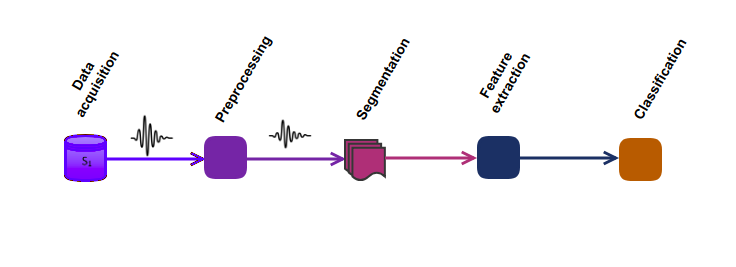
\includegraphics[width=.6\textwidth]{Figures/HARP.png}
    \caption{Human activity recognition process}
    \label{fig:tsprocess}
\end{figure}

ARP is composed of a sequence of signal processing, pattern recognition, and 
machine learning techniques~\cite{bulling2014tutorial}. It mainly 
consists of 5 steps, shown in Figure \ref{fig:tsprocess} and 
explained hereafter.

\begin{figure}[ht]
    \centering
    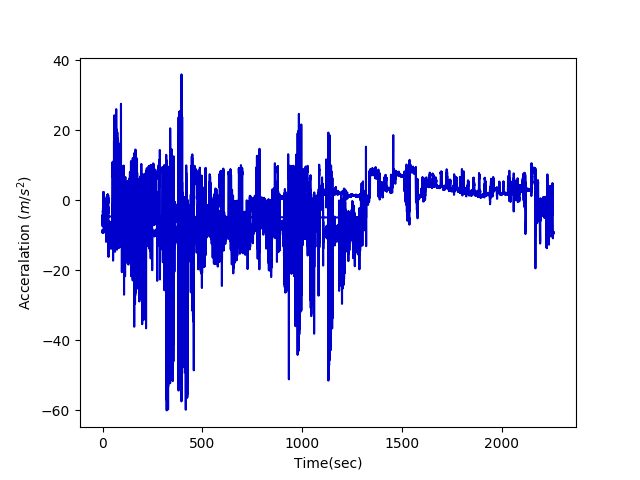
\includegraphics[width=.4\textwidth]{Figures/signal.png}
    \caption{Example acceleration data extracted from~\cite{banos2012benchmark}.}
    \label{fig:signal}
\end{figure}
\noindent\textbf{Data acquisition.} Several sensors are attached to different body parts. They mostly acquire 3D acceleration, gyroscopic and magnetic field measurements, as shown in Figure~\ref{fig:signal}. Sensors discretize signals at a given frequency, typically 50Hz for 
daily activities or 200Hz for fast sports, and transmit the resulting data points to 
the receiver. 

\noindent\textbf{Pre-processing.} Data points coming from sensors may
include artifacts of various origins such as 
electronic fluctuations, sensor malfunctions, and physical activities~\cite{arlot2010survey}. To eliminate such artifacts, filtering techniques are commonly applied, such as the Butterworth low-pass filter, which flats the coming signals as much as possible through rolling off down the higher frequencies beyond the cut-off point to zero ~\cite{morris2014recofit,selles2005automated,najafi2003ambulatory}. 
Filtering should be used with care as it may also remove valuable information from the signals.


\noindent\textbf{Segmentation.}
Discrete data points produced by the sensors are partitioned into time 
windows labeled from the most frequent activity in the window. The number of data 
points in a time window, a.k.a the window size, heavily impacts the 
performance of the model~\cite{bulling2014tutorial,banos2014window}. Finding the optimal window size depends on the specific requirements of the HAR system. For instance, the number of activities for which system is devised or special recognition time~\cite{banos2014window}. However, in any case, the window size should be properly selected in such a way that each window contains enough samples(at least one cycle of an activity) to be differentiable from similar movements~\cite{janidarmian2017comprehensive}. The current method 
to select the window size is empirical~\cite{bulling2014tutorial}. People apply ARP with different window sizes which mostly selected from the values used in previous works, and choose the one which maximizes the performance of the recognition system. This process can be very time consuming due to the fact that there is no prior knowledge about the optimal window size and the whole space should be searched in an uninformed way.  


\noindent\textbf{Feature extraction.}
Each time window is then transformed into a vector of features such as auto-correlation features~\cite{morris2014recofit}, or statistical 
moments. These features are then used to help discriminate various activities.

\noindent\textbf{Classification.}
Finally, a classifier is trained on the vector of features and corresponding 
labels, and assigns future 
observations to one of the learned activities. According to~\cite{lara2013survey}, Decision trees, Naive Bayes, SVM, k-nearest neighbors, Hidden Markov Models and ensemble classifiers such as Random Forest are the most important classifiers in HAR.

The window size in the segmentation step and the feature selection in feature extraction step are hyperparameters of the ARP, usually 
selected by trial and error as in~\cite{banos2014window}.

    

\subsection{Sliding windows technique}

\begin{figure}[htp]
\captionsetup[subfigure]{justification=centering}

  \centering
  \subfigure[Non-overlapping]{
\label{subfig:NOSW}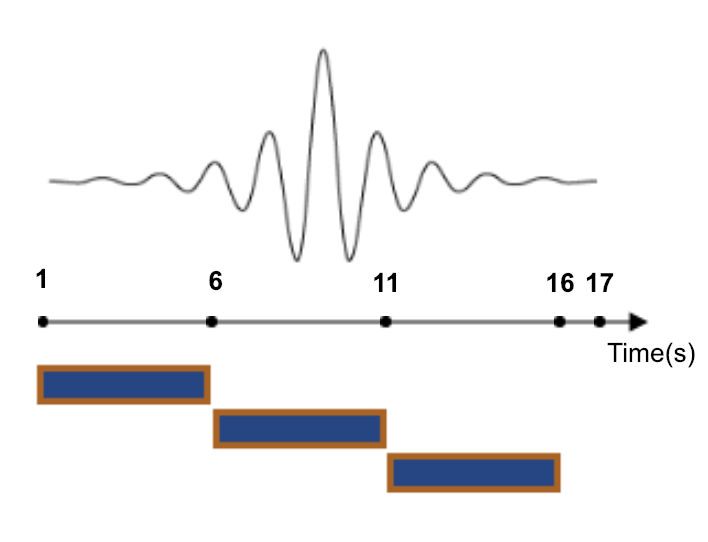
\includegraphics[scale=0.4]{Figures/NOSW.png}}\quad
  \subfigure[Overlapping-2 s sharing ]{\label{subfig:OSW}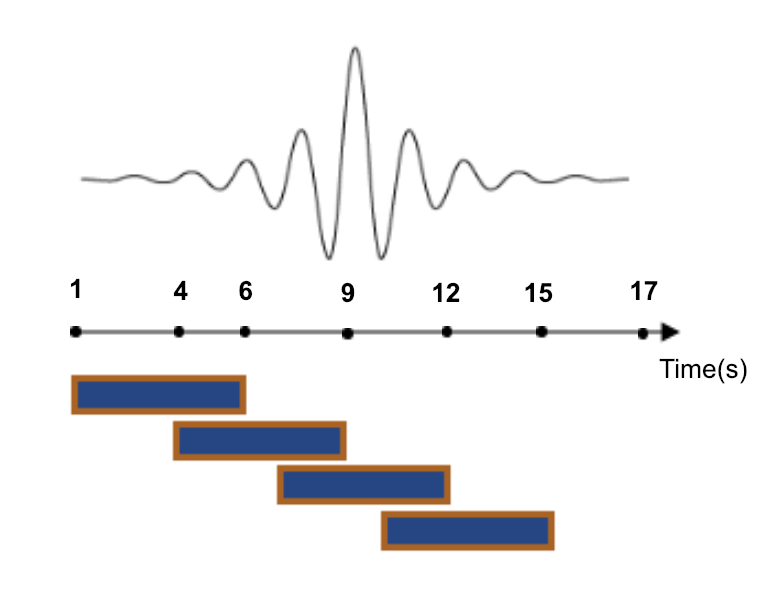
\includegraphics[scale=0.4]{Figures/OSW.png}}

   \caption{5-second sliding windows. }
   \label{fig:SlidingWindow}
\end{figure}

In the segmentation step of ARP, the data points are partitioned into segments of data to capture the dynamics of activities. This process assumes that each 
window is an approximation of the signal for which the classifier will 
have to make a decision. There are several ways to segment the sensor signals in HAR field which can be categorized into three groups, namely activity-defined windows, event-defined windows and sliding windows~\cite{banos2014window}. The sliding window approach is the most widely used method in segmentation step of ARP. In this approach, the sensor signals are split into windows of fixed size. If there are overlap between adjacent windows, this technique is known as overlapping sliding window, and if not, it is called non-overlapping windows technique. 
Figure~\ref{fig:SlidingWindow} illustrates the 
non-overlapping and overlapping windowing techniques.
There is a generalized idea that using overlapping sliding windows increases the performance of classifiers in HAR~\cite{janidarmian2014automated}, since they involve more data points, and unlike the non-overlapping windows, they are not prone to missing important events~\cite{coggeshall2005asset}, particularly within activity transition periods. While these assumptions are generally true, we will show later with our detailed experiments that non-overlapping windows overall deliver comparable recognition accuracy, while majorly reducing the required training computations and memory usage.
\subsection{System evaluation}
\label{sub:CVs}
One of the most important step in designing each system is evaluation. The evaluation in HAR has been mostly carried out through k-fold CV. In k-fold CV (Figure~\ref{fig:Shuffle-cv}), the overall data is randomly partitioned in $k$ equal subsets. The model is then trained on $k-1$ subsets, and the remaining one is used for testing~\cite{trevor2009elements}. In this process, the test set can be any part of the dataset meaning that training and test sets may contain the data of same subject and due to that, this method is referred to as subject-dependent CV in literature~\cite{al2019deep}.  
The main assumption of this process is that \emph{samples are Independent and Identically Distributed (i.i.d.)}~\cite{arlot2010survey}, which means that all the data points are sampled independently from the same distribution.  However, samples drawn from a given subject are likely to \emph{not} be independent, for two reasons. First, there is a strong inter-subject variability in the way activities are conducted~\cite{bulling2014tutorial}. This means that the similarity of samples drawn from the same subject is likely to be higher than that of samples drawn from different subjects. Several factors might explain such variability, including sex, gender, age or experience. Second, there is a temporal dependence between activities performed by the same subject: the similarity between samples drawn in a short time interval, for instance in the same training session in case of training activities, will most likely be higher than that of samples drawn further apart in time. This is due to factors such as fatigue and training. Thus, k-fold CV may overestimate the performance of recognizer systems in HAR. Such overestimation is even larger when k-fold CV is used with overlapping sliding windows since the overlap between adjacent windows is another source of dependency between data points. A more formal discussion about the problems of k-fold CV in HAR can be found in~\cite{dehghani2019subject}.   

% this method overstimate and it increases when the overlap increase

To address these issues, the training and testing sets should be splitted by subject. In this method which is known as subject-independent CV~\cite{al2019deep,janidarmian2017comprehensive}, in each iteration the model is trained on all the subjects except one, which is used for testing. In this way, the intra-subject dependencies present in subject-dependent CV are hence removed. It should be noted that, in this case, as is shown in Figure~\ref{fig:Subjective-cv}, the number of folds is lower or equal to the number of subjects in the dataset.    


\begin{figure}[htp]
  \centering
  \subfigure[Subject-dependent CV]
  {\label{fig:Shuffle-cv}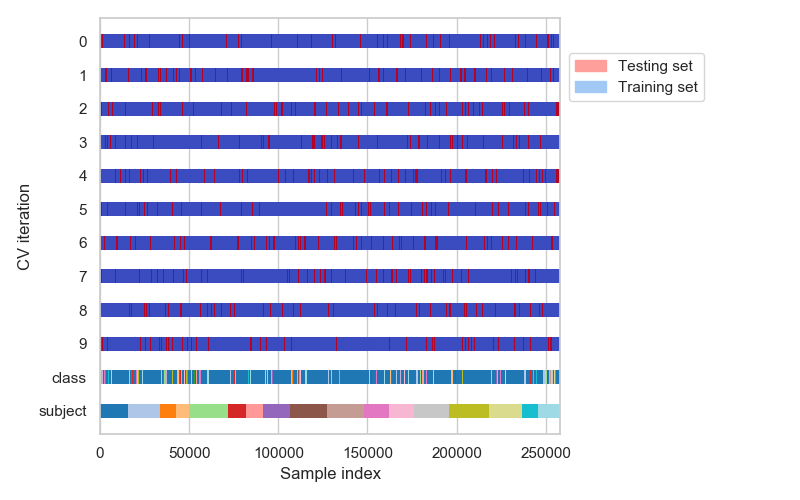
\includegraphics[scale=0.37]{Figures/ShuffleSplit.png}}\quad
  \subfigure[Subject independent CV]
  {\label{fig:Subjective-cv}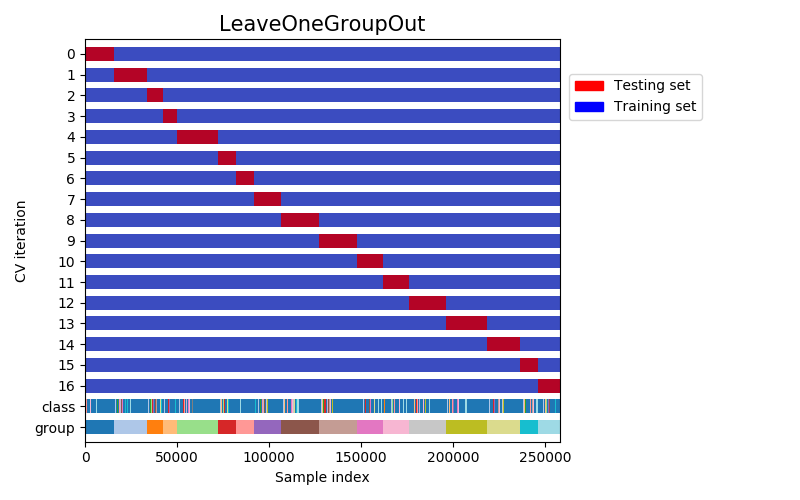
\includegraphics[scale=0.37]{Figures/LeaveOneGroupOut.png}}
   \caption{Different types of CV in HAR}
    \label{fig:CVs}
\end{figure}




\section{Datasets and Experimental Setup} \label{sec:experiment setting}
\subsection{Datasets} \label{sec:dataset}
In this study, we use two public datasets of human activity, to evaluate the impact of overlapping windows in a wide range of subjects, activities, and conditions. 

\noindent\textbf{Dataset 1.} \label{sec:dataset1}
 As the first dataset, we use the dataset described in~\cite{banos2012benchmark}, one of the most complete public datasets for HAR in terms of the number of activities and subjects. The dataset consists of data collected from 17 subjects of diverse profiles while wearing 9 Xsens\footnote{\url{https://www.xsens.com}} inertial measurement units (IMU) on different parts of their body. Subjects performed 33 fitness activities (Table \ref{tab:Activites1}) ranging from warm up to fitness exercises in an out-of-lab environment. Each sensor provides tri-directional acceleration, gyroscope, and magnetic field measurements, as well as, orientation estimates in quaternion format (4D). Similar to prior work in~\cite{banos2014window}, acceleration data was used in our study. The dataset also provides data for three sensor displacement scenarios namely ``default", ``self-placement" and ``mutual-displacement" to compare the sensor anomalies, but as in~\cite{banos2014window}, only the data from default scenario is used in our study. 

%  start of Table1
\begin{table}
  \centering
\begin{tabular}{|c|c|}
\hline 
\multicolumn{2}{|c|}{Activities}\tabularnewline
\hline 
\hline 
Walking (1 min) & Upper trunk and lower body opposite twist (20x)\tabularnewline
\hline 
Jogging (1 min) & Arms lateral elevation (20x)\tabularnewline
\hline 
Running (1 min) & Arms frontal elevation (20x)\tabularnewline
\hline 
Jump up (20x) & Frontal hand claps (20x)\tabularnewline
\hline 
Jump front \& back (20x) & Arms frontal crossing (20x)\tabularnewline
\hline 
Jump sideways (20x) & Shoulders high amplitude rotation (20x)\tabularnewline
\hline 
Jump leg/arms open/closed (20x) & Shoulders low amplitude rotation (20x)\tabularnewline
\hline 
Jump rope (20x) & Arms inner rotation (20x)\tabularnewline
\hline 
Trunk twist (arms outstretched) (20x) & Knees (alternatively) to the breast (20x)\tabularnewline
\hline 
Trunk twist (elbows bended) (20x) & Heels (alternatively) to the backside (20x)\tabularnewline
\hline 
Waist bends forward (20x) & Knees bending (crouching) (20x)\tabularnewline
\hline 
Waist rotation (20x) & Knees (alternatively) bend forward (20x)\tabularnewline
\hline 
Waist bends (reach foot with opposite hand) (20x) & Rotation on the knees (20x)\tabularnewline
\hline 
Reach heels backwards (20x) & Rowing (1 min)\tabularnewline
\hline 
Lateral bend (10x to the left + 10x to the right) & Elliptic bike (1 min)\tabularnewline
\hline 
Lateral bend arm up (10x to the left + 10x to the right) & Cycling (1 min)\tabularnewline
\hline 
Repetitive forward stretching (20x) & \tabularnewline
\hline 
\end{tabular}
      % Title of the table
        \caption{Activity set in the dataset 1.}        
        \label{tab:Activites1}
\end{table} 


\noindent\textbf{Dataset 2.} \label{sec:dataset2}
The second dataset used is also one of the most complete and big public datasets for HAR in terms of the number of activities and subjects~\cite{morris2014recofit}. The dataset contains data for 74 activities (Table~\ref{tab:Activites2}) from 94 subjects (28 female), ages 18-58 ($\mu=34.2$). Data was collected in a large lab space from an armband worn on the right forearm, containing a SparkFun “Razor IMU” inertial sensor\footnote{\url{https://www.sparkfun.com}}. This IMU includes a 3-axis accelerometer and a 3-axis gyroscope which transmit sensor values to a PC at 50Hz. As can be seen in Table~\ref{tab:Activites2}, there are several activities in the dataset such as "Arm band adjustment" and "Device on Table" which we consider as noise in this study. Besides, since during the data collection, the subjects wore a single joint sensor on their right forearm, the activities of the opposite hand (left hand) can not be captured properly with the sensors. Thus, we have done a relabeling process to clarify the dataset. In this process, (1) we label all the irrelevant and opposite hand activities as a "Noise" class (2) all the activities that refer to multiple labels are grouped together as one exercise. Table~\ref{tab:Activites2} shows all the activities and their labels after the relabeling process.   

\begin{table}
\setlength\tabcolsep{1pt}
    \small
    \centering
%\footnotesize\setlength{\tabcolsep}{2.5pt}

\begin{tabular}{|c|c|c|c|c|c|}
\hline 
Activity & Label & Activity & Label & Activity & Label\tabularnewline
\hline 
Arm band adjustment & 1(Noise) & Lawnmower (both) & 20 & Squat (arms in front) & 33\tabularnewline
\hline 
Arm straight up & 1(Noise) & Lawnmower (left) & 1(Noise) & Squat (hands behind head) & 33\tabularnewline
\hline 
Band Pull-Down row & 2 & Lawnmower (right) & 21 & Squat (kettlebell) & 33\tabularnewline
\hline 
{}Bicep Curl & 3 & Lunge (both legs) & 22 & Squat Jump & 33\tabularnewline
\hline 
Bicep Curl (band) & 3 & Ball Slam & 23 & Squat Rack Shoulder Press & 33\tabularnewline
\hline 
Box Jump & 4 & No Exercise & 1(Noise) & Static Stretching & 1(Noise)\tabularnewline
\hline 
Burpee & 5 & Note & 1(Noise) & Stretching & 1(Noise)\tabularnewline
\hline 
Butterfly sit-up & 6 & {}Triceps Extension(standing) & 24 & Tap IMU & 1(Noise)\tabularnewline
\hline 
Chest Press & 7 & Triceps Extension (both) & 24 & Tap left IMU & 1(Noise)\tabularnewline
\hline 
Crunch & 8 & Plank & 25 & Tap right IMU & 1(Noise)\tabularnewline
\hline 
Device on Table & 1(Noise) & Power Boat pose & 26 & Triceps Kickback(bench --both) & 34\tabularnewline
\hline 
Dip & 9 & Pushups (foot variation) & 27 & Triceps Kickback (bench --left) & 1(Noise)\tabularnewline
\hline 
Dumbbell Deadlift Row & 10 & {}Pushups & 27 & Triceps Kickback (bench --right) & 34\tabularnewline
\hline 
{}Dumbbell Row (both) & 11 & Stretching & 1(Noise) & {}Triceps Extension (lying --both) & 35\tabularnewline
\hline 
Dumbbell Row (left) & 1(Noise) & Rest & 1(Noise) & Triceps Extension (lying --left) & 1(Noise)\tabularnewline
\hline 
Dumbbell Row (right) & 12 & Rowing Machine & 28 & Triceps Extension (lying --right) & 35\tabularnewline
\hline 
Dumbbell Squat (hands at side) & 13 & Running & 29 & Two-arm Dumbbell Curl (both) & 36\tabularnewline
\hline 
Dynamic Stretch & 1(Noise) & Russian Twist & 30 & Non-listed & 1(Noise)\tabularnewline
\hline 
Elliptical Machine & 14 & Seated Back Fly & 31 & V-up & 37\tabularnewline
\hline 
Punches & 15 & {}Shoulder Press & 32 & Walk & 38\tabularnewline
\hline 
Invalid & 1(Noise) & Side Plank (left) & 25 & Walking lunge & 39\tabularnewline
\hline 
Jump Rope & 16 & Side Plank (right) & 25 & Wall Ball & 40\tabularnewline
\hline 
Jumping Jacks & 17 & Sit-up (hand behind head) & 6 & Wall Squat & 41\tabularnewline
\hline 
Kettlebell Swing & 18 & Sit-up & 6 & Dumbbell Curl (alternating) & 36\tabularnewline
\hline 
{}Lateral Raise & 19 & Squat & 33 &  & \tabularnewline
\hline 
\end{tabular}
    \caption{Activity set in the dataset 2.}
    \label{tab:Activites2}
\end{table}

\subsection{Experimental Setup} \label{sec:experiment setup}
Similar to prior work~\cite{banos2014window}, we did not apply any pre-processing to the dataset. We used both overlapping and non-overlapping windows. Overlapping windows were sliding at 200~ms, with window sizes ranging from 0.25~s to 7~s in steps of 0.25 s. For instance, a 5-second window shared 4.8~s of data with the previous one. For non-overlapping windows, we used the same settings as in~\cite{banos2014window}: disjoint windows with sizes ranging from 0.25~s to 7~s in steps of 0.25 s. We used the same feature sets as in~\cite{banos2014window}, namely FS1 (mean only), FS2 (mean and standard deviation) and FS3 (mean, standard deviation, maximum, minimum and mean crossing rate). Finally, for the classification part, we used the following classifiers: Decision Tree (DT), K-nearest neighbors (KNN, K=3), Naive Bayes (NB), Nearest Centroid Classifier (NCC). We used these classifiers as implemented in scikit-learn 0.20~\cite{pedregosa2011scikit} with default hyperparameters.
 
 To evaluate model performance, we used both subject-dependent CV and subject-independent CV. We use the F1-score as performance measure due to its robustness in class imbalance. F1-score which reaches its best at 1 and worse at 0, is computed as follows:
 \begin{center}
      $F1= \frac{2\times(precision \times recall)}{(precision + recall)}$
 \end{center}

All the source codes for conducted experiments are available in our GitHub repository \footnote{\url{http://www.github.com/big-data-lab-team/paper-generalizability-window-size}}. It contains the scripts to segment the datasets for different window sizes, feature sets and sliding window techniques. There is also a script for training and testing all mentioned classifiers on windowed datasets. Finally it also contains code to reproduce all presented figures in this paper.
%%%%%%%%%%%%%%%%%%%%%%%%%%%%%%%%%%%%%%%%%%
\section{Results} \label{sec:result}
In this section, the impact of the overlapping and non-overlapping sliding windows in HAR systems with Subject-dependent CV and Subject-independent CV for both datasets is evaluated. We report distributions of  F1-score values across window sizes, we plot the distribution of the F1-scores, so as to  visually compare the classifiers performances in overlapping and non-overlapping sliding windows techniques. The experiments are categorized into global evaluation and activity-specific analysis.

\subsection{Global evaluation}\label{global_evaluation}
In these set of experiments, we analyze the general impact of overlapping and non-overlapping windowing in HAR systems trough the average performance of models for different activities and window sizes. 
\subsubsection{Experiment 1: Subject-dependent CV} \label{sec:ex1}
In this experiment, we apply non-overlapping and overlapping windowing with Subject-dependent CV and use it as a baseline
for further evaluations. 

We applied the ARP system as explained in Section~\ref{sec:experiment setup}, on the datasets described in Section~\ref{sec:dataset}. For each window size, we partitioned the dataset in non-overlapping and overlapping windows separately and extracted feature sets FS1, FS2, and FS3 in each window. We trained the classifiers on the resulting feature vectors, and measured their average F1-score over 10-fold CV.

\noindent\textbf{Dataset 1}- Figure~\ref{fig:exp1_ds1} shows the distribution of the F1-scores of the classifiers for different window sizes in overlapping and non-overlapping windows. The classifiers can be categorized in two groups: (1) KNN and DT, that have very different performance distributions for overlapping and non-overlapping windowing, and (2) NB and NCC, that show almost similar distributions for both techniques. Our findings show that, in general, using overlapping windowing improves the performance of all classifiers in all feature sets. Regarding the first group, quantitatively, using the overlapping windowing technique improves the F1-score of the KNN and DT about 10\%, 8\% and 8\% on average in FS1, FS2, and FS3 respectively. However, the improvement for the second group is about 1\%, on average, for all features sets, which is insignificant.

\noindent\textbf{Dataset 2}- The distribution of F1-scores for different window sizes and classifiers for overlapping and non-overlapping windowing is shown in Figure~\ref{fig:exp1_ds2}. Generally, the trends for Dataset 2 and Dataset 1 are similar. Overlapping windowing increases the F1-score and we observe the same two performance groups as before. The F1-score distributions of DT and KNN for overlapping and non-overlapping windowing are very different. Quantitatively, using overlapping sliding windows increases the performance of KNN and DT about 9\%, 12\% and 13\% on average in FS1, FS2, and FS3 respectively. Regarding the NB and NCC, however, the increase is minor to negligible for all feature sets. 

These results show that using the overlapping windowing technique rather than non-overlapping one in subject-dependent CV can improve the performance of classifiers. This agreement between our results and the general argument of the effectiveness of overlapping windowing in HAR systems~\cite{janidarmian2017comprehensive,janidarmian2014automated}
reinforces our confidence in the correctness of our analysis method and its applicability for next experiments.  



\subsubsection{Experiment 2: subject-independent CV} \label{sec:ex2}
As described in Section~\ref{sub:CVs},  subject-independent CV should be used to evaluate the performance of HAR systems. Thus, in this experiment, we compare the overlapping and non-overlapping windowing techniques when using subject-independent CV.  

The only difference between this experiment and Experiment 1 is the use of subject-independent CV rather than subject-dependent CV.

\noindent\textbf{Dataset 1}- Figure~\ref{fig:exp2_ds1} shows our results. Similar to Experiment 1 for this dataset, we observed the same two performance groups. Regarding the first group, however, the F1-score differences among groups are very tiny. Contrary to Experiment 1, using overlapping windowing decreases the F1-scores of DT and KNN in all feature sets. Qualitatively, differences for DT and KNN in overlapping and non-overlapping windowing are about 0.02\%, 0.04\% and 0.01\% on average in FS1, FS2, and FS3 respectively, which are practically negligible improvements.  
As for the second group, the performances of NB and NCC are almost the same in all feature sets. 

\noindent\textbf{Dataset~2}- Figure~\ref{fig:exp2_ds2} shows the results of Experiment~2 for Dataset~2. In spite of having the same two performance groups as in Experiment~1, here the F1-scores for overlapping and nonoverlapping are very similar.
%In general, using overlapping instead of nonoverlapping, except for FS1-NCC and FS3-NB, windowing increases the performance of classifiers slightly for in all feature sets.
In particular, DT and KNN with overlapping windowing shows about 0.02\%, 0.01\% and 0.01\% performance improvement on average in comparison to using them with non-overlapping windowing. For NB and NCC the F1-scores of both techniques are similar for all feature sets.

In general, compared to Experiment~1 for both datasets, the performance of all classifiers in all feature sets decreased which may be resulted from the overestimation of Subject-dependent CV. On the other words, subject-independent CV removes the performance improvement resulting from using overlapping windows in Experiment~1 which seems to be resulted from the overestimation of subject-dependent CV. This experiment represents that the performance advantage of overlapping windows in the literature seems to be resulted from the use of subject-dependent CV and in case of using subject-independent CV, this method does not offer any benefit to the performance of HAR systems. Hence, we can reach to the same recognition performance by using non-overlapping windows. Considering the resource-intensity of overlapping windowing compared to non-overlapping one,  this is an important conclusion since through that we can save a lot of resources (energy, time, etc) which is a desirable feature in HAR~\cite{lara2012survey}.   



\begin{figure}[htp]
  \centering
  \subfigure[FS1]{\label{fig:ds1-FS1-exp1}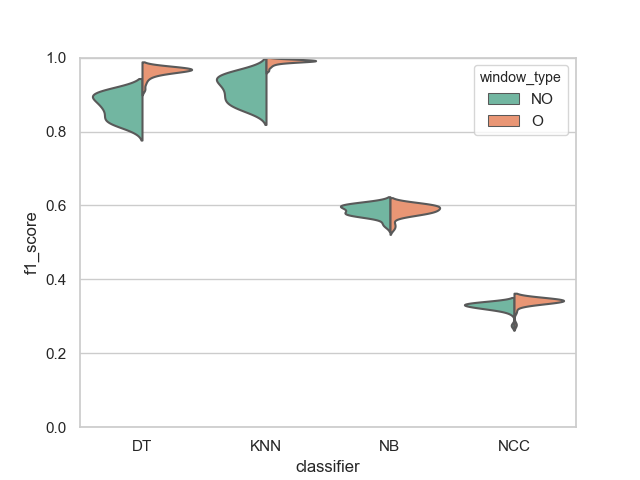
\includegraphics[scale=0.31]{Figures/banos_iid_FS1.png}}\quad
  \subfigure[FS2]{\label{fig:ds1-FS2-exp1}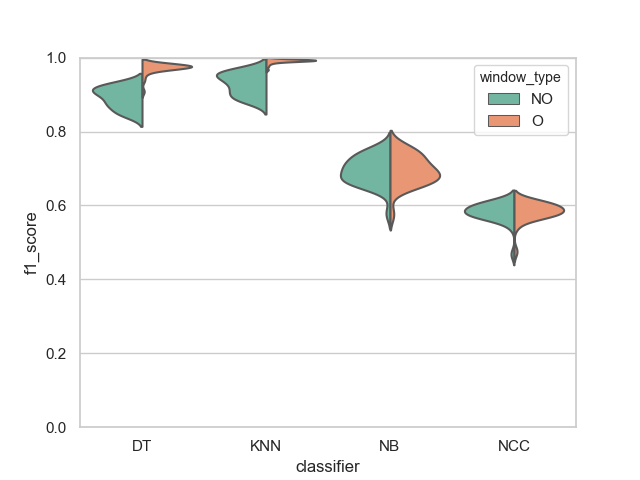
\includegraphics[scale=0.31]{Figures/banos_iid_FS2.png}}
  \subfigure[FS3]{\label{fig:ds1-FS3-exp1}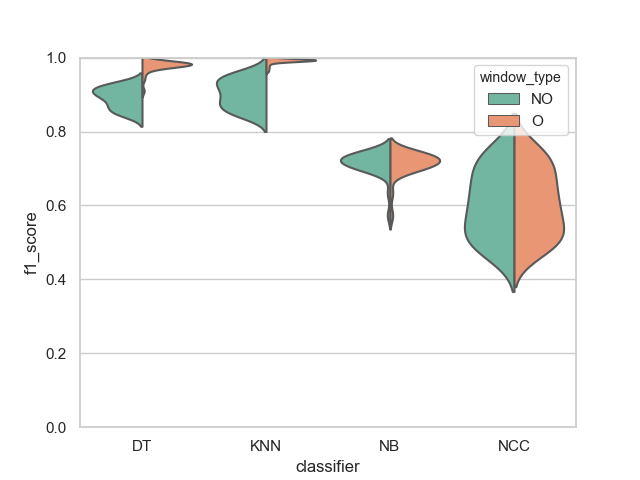
\includegraphics[scale=0.31]{Figures/banos_iid_FS3.png}}
   
   \caption{Experiment 1 -- Subject-dependent CV -- Dataset 1. O and NO stand for overlapping and non-overlapping windowing respectively.}
    \label{fig:exp1_ds1}
    
\end{figure}

\begin{figure}[htp]
  \centering
  \subfigure[FS1]{\label{fig:ds2-FS1-exp1}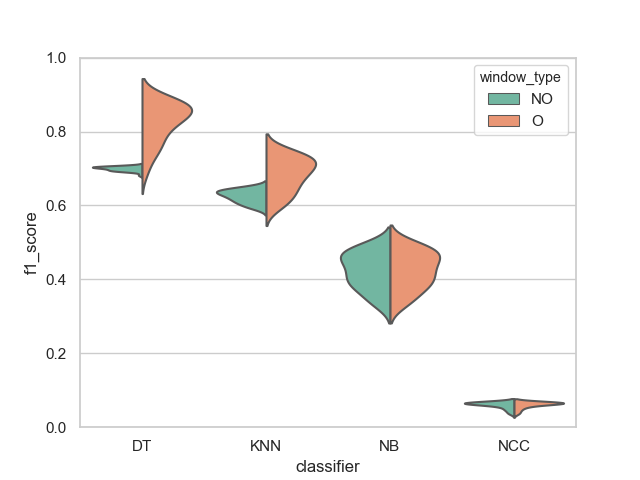
\includegraphics[scale=0.31]{Figures/recofit_iid_FS1.png}}\quad
  \subfigure[FS2]{\label{fig:ds2-FS2-exp1}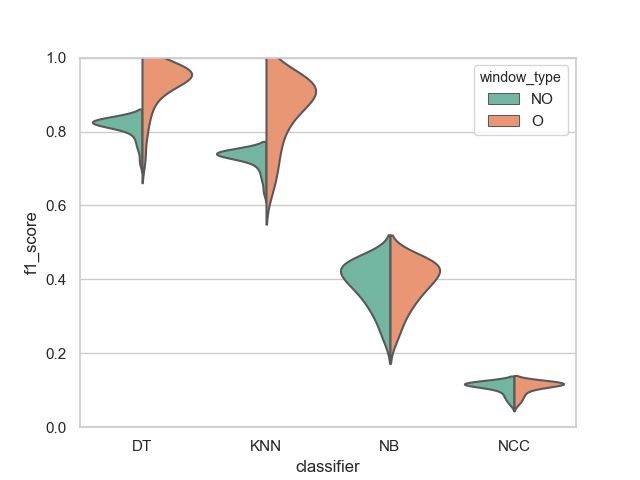
\includegraphics[scale=0.31]{Figures/recofit_iid_FS2.png}}
  \subfigure[FS3]{\label{fig:ds2-FS3-exp1}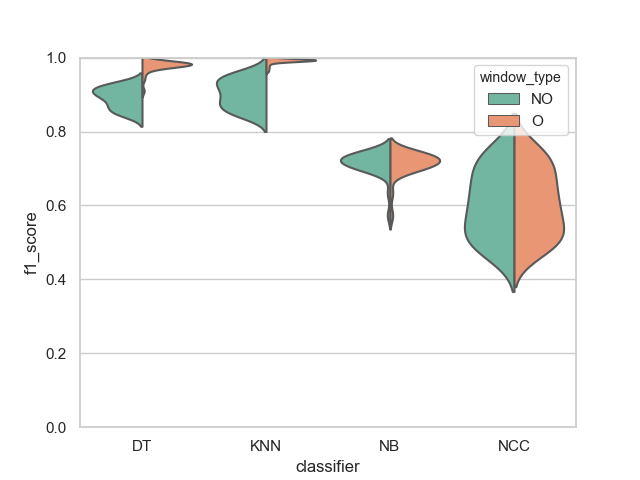
\includegraphics[scale=0.31]{Figures/recofit_iid_FS3.png}}
   
   \caption{Experiment 1 -- Subject-dependent CV -- Dataset 2. O and NO stand for overlapping and non-overlapping windowing respectively.}
    \label{fig:exp1_ds2}
    
\end{figure}

\begin{figure}[htp]
  \centering
  \subfigure[FS1]{\label{fig:ds1-FS1-exp2}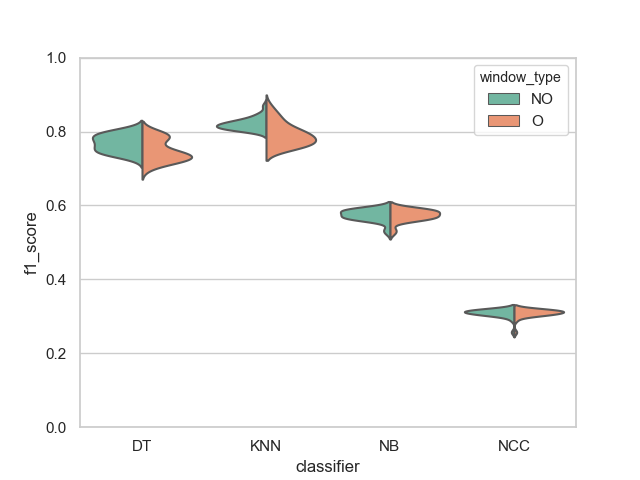
\includegraphics[scale=0.31]{Figures/banos_sbj_FS1.png}}\quad
  \subfigure[FS2]{\label{fig:ds1-FS2-exp2}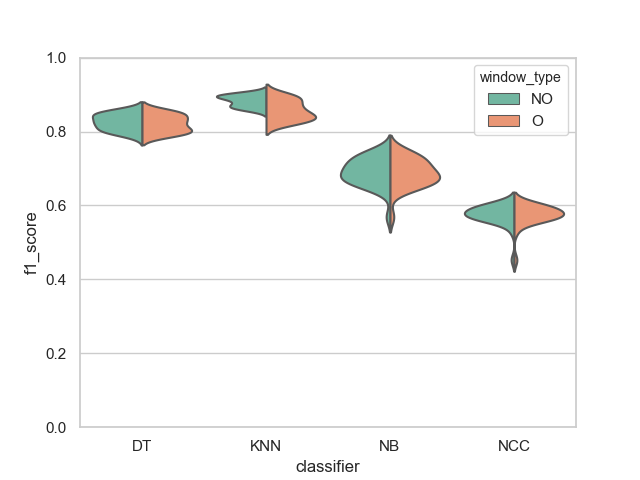
\includegraphics[scale=0.31]{Figures/banos_sbj_FS2.png}}
  \subfigure[FS3]{\label{fig:ds1-FS3-exp2}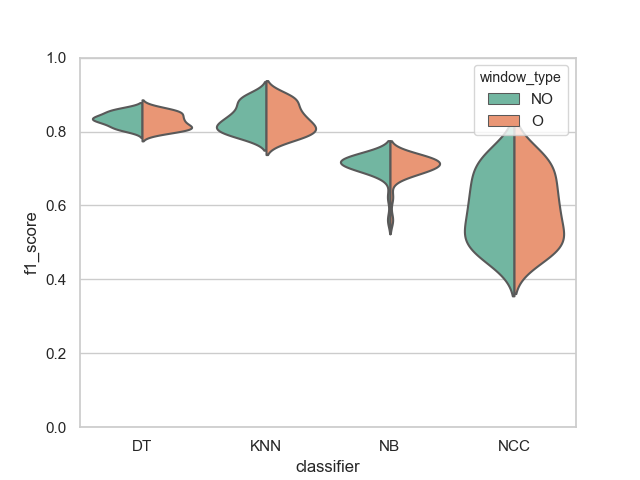
\includegraphics[scale=0.31]{Figures/banos_sbj_FS3.png}}
   
   \caption{Experiment 2 -- Subject-independent CV -- Dataset 1. O and NO stand for overlapping and non-overlapping windowing respectively.}
    \label{fig:exp2_ds1}
    
\end{figure}

\begin{figure}[htp]
  \centering
  \subfigure[FS1]{\label{fig:ds2-FS1-exp2}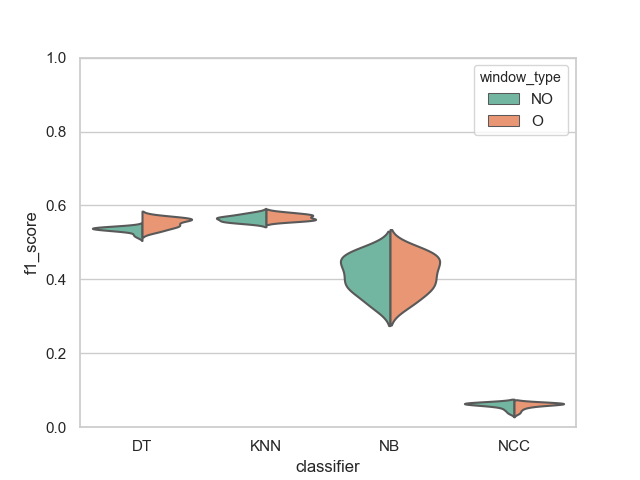
\includegraphics[scale=0.31]{Figures/recofit_sbj_FS1.png}}\quad
  \subfigure[FS2]{\label{fig:ds2-FS2-exp2}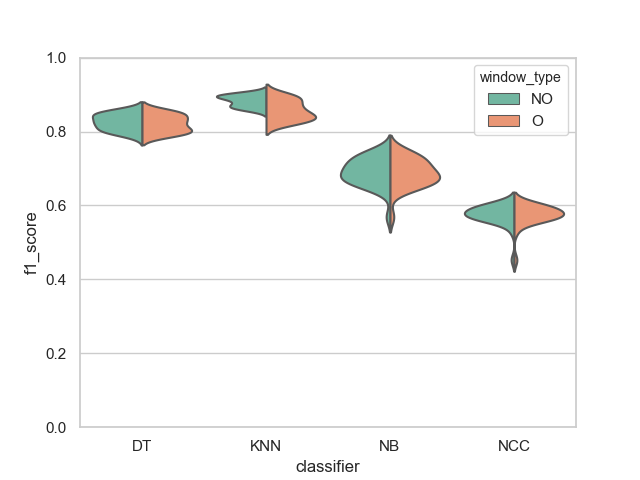
\includegraphics[scale=0.31]{Figures/recofit_sbj_FS2.png}}
  \subfigure[FS3]{\label{fig:ds2-FS3-exp2}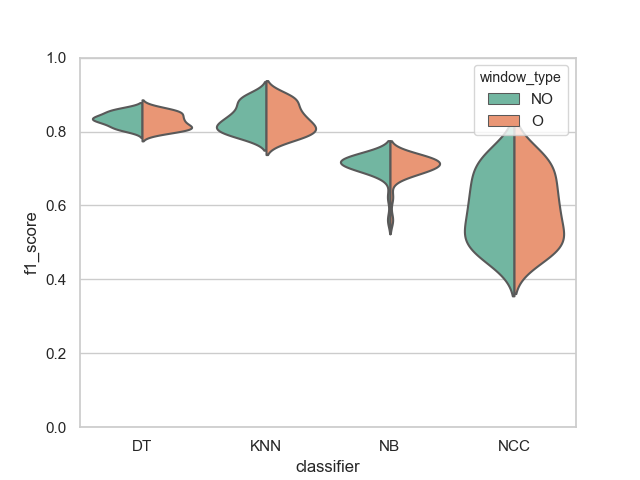
\includegraphics[scale=0.31]{Figures/recofit_sbj_FS3.png}}
   
   \caption{Experiment 2 -- Subject-independent CV -- Dataset 2. O and NO stand for overlapping and non-overlapping windowing respectively.}
    \label{fig:exp2_ds2}
    
\end{figure}

\subsection{Activity-Specific evaluation}\label{per_activity_evaluation}
The global evaluation presented previously is useful to have a general view of the effect of windowing techniques in HAR systems. However, it is also interesting to particularize this study to each specific activity. Thus, in this section, we analyze the impact of overlapping and non-overlapping windowing for each activity.

\subsubsection{Experiment 3: Subject-independent CV}
As discussed in Section~\ref{sec:ex2}, there is a slight difference in the performance of classifiers for overlapping and non-overlapping windowing techniques. Thus, in this experiment, we apply such techniques with subject-independent CV to investigate the source of such differences. 
For brevity, we only focus on feature set FS3.

\noindent\textbf{Dataset 1}- In Figure~\ref{fig:exp3_ds1}, the activity-specific F1-scores distributions achieved for all classifiers, window sizes and windowing approaches are presented. As expected from the results shown in~\ref{fig:ds1-FS3-exp2}, the differences between overlapping and non-overlapping windowing for all activities are slight. In general, the performances of the majority of the activities drop when overlapping windowing instead in of non-overlapping is used. Regarding the DT, in Figure~\ref{fig:DT_ds1-activity-exp3}, activities such as Heels, Rotation on knees, Trunk Twist, Knees (altering), Knees Bending, Rowing and Jump rope show improvement by overlapping windowing. In spite of being small, on average for all window sizes, Heels and Lateral elevation of arms by 0.06\% reduction and growth respectively, show the highest differences between overlapping and non-overlapping windowing. As for KNN (Figure~\ref{fig:KNN_ds1-activity-exp3}), improvements by using overlapping are inconsiderable (<0.03\% ). However, quantitatively,  reductions are higher than DT. As an example, using overlapping drops the performance of  Repetitive forward stretching by 0.11\% which is significant. This may be due to the nature of this classifier~\cite{cover1967nearest}, for which small change in the dataset may have a large impact on the performance. As can be seen in Figure~\ref{fig:NB_ds1-activity-exp3} and Figure~\ref{fig:NCC_ds1-activity-exp3}, the performance of all activities for NB and NCC are almost the same.    

\noindent\textbf{Dataset 2}- Our results for this experiment are shown in Figure~\ref{fig:exp3_ds2}. In general, based on the performance of the classifiers, this dataset seems to be more challenging in comparison to Dataset~1. Particularly, in short window sizes (< 5s), the obtained F1-scores for most of the activities are low. It may be due to the fact that in comparison to Dataset~1 which are collected from 9 IMUs, only one IMU is used for collecting this dataset. It is proven that in the case of using multiple IMU, we can achieve reasonable performance even in short window sizes~\cite{banos2014window}. Furthermore, the number and complexity of activities in Dataset~2 are higher compared to Dataset~1. As in the results for Dataset~1, the activity-specific F1-score distributions obtained for this dataset for two scenarios are similar. However, in spite of being negligible, using overlapping windowing slightly enhances the F1-score of the majority of activities in comparison with non-overlapping one for KNN and DT. Particularly, most improvements are observed in Lawnmower (right arm), Lateral Raise and Seated Back Fly activities for DT and Wall Ball, Seated Back Fly and Power Boat pose for KNN by about 0.05\% on average. Similar to Dataset~1, the performance of NB and NCC for all activities in both scenarios are almost the same. 

This experiment shows that using overlapping windowing with subject-independent can impact the recognition performance of HAR systems for diverse activities differently. In spite of being mostly minor, for the activities in this study, overlapping windowing reduces the recognition accuracy of the most activities and only a few of them shows improvement. Moreover, the impact of overlapping windowing may be subject to the dataset, i.e., using overlapping windowing may impact the performance of the system in recognizing a single activity in different way. Running is a good example here. Using overlapping windowing reduces the F1-score of the system for this activity in Dataset~1, but it improves that in Dataset~2.  

On the other words, some  
the performance of the recognition systems for most of the activities investigated in this study drops when overlapping windowing instead of non-overlapping one is used.    


\begin{figure}[htp]
  \centering
  \subfigure[DT]{\label{fig:DT_ds1-activity-exp3}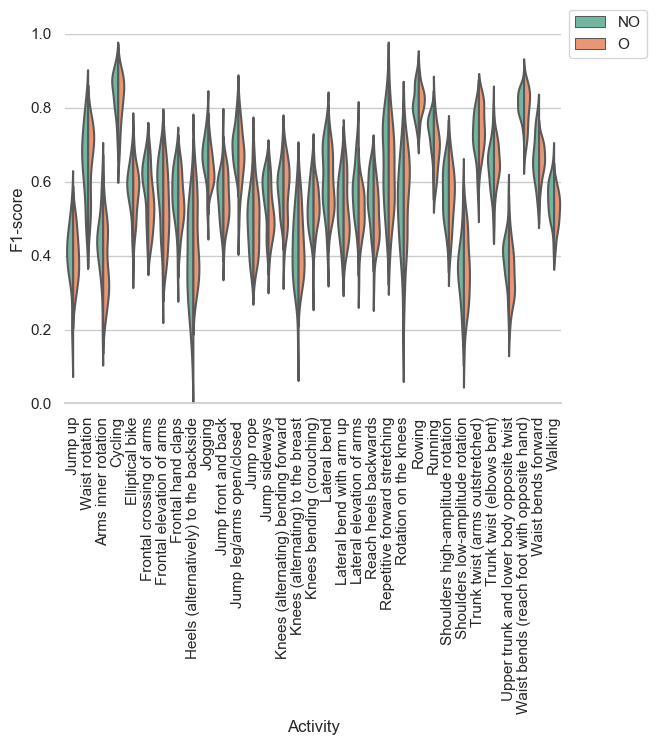
\includegraphics[scale=0.4]{Figures/per_activity_DT_banos_sbj_FS3.png}}\quad
  \subfigure[KNN]{\label{fig:KNN_ds1-activity-exp3}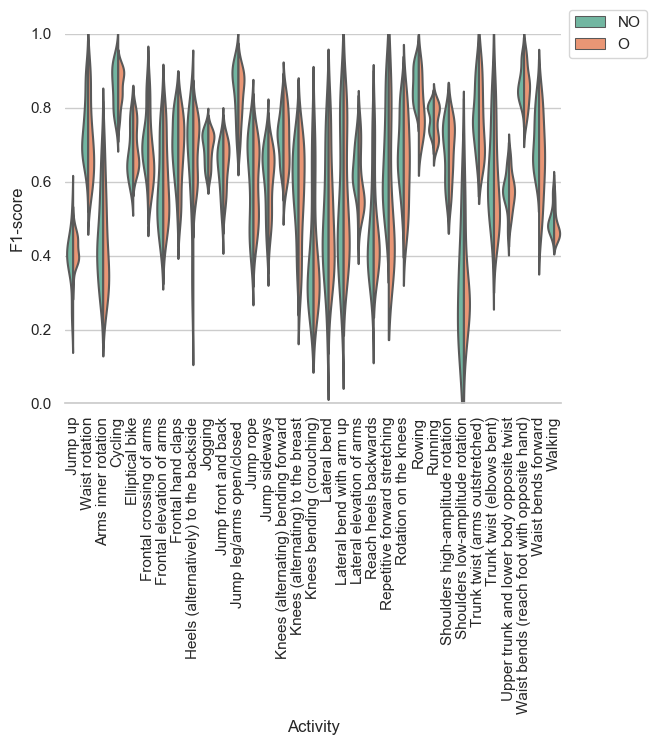
\includegraphics[scale=0.4]{Figures/per_activity_KNN_banos_sbj_FS3.png}}
  \subfigure[NB]{\label{fig:NB_ds1-activity-exp3}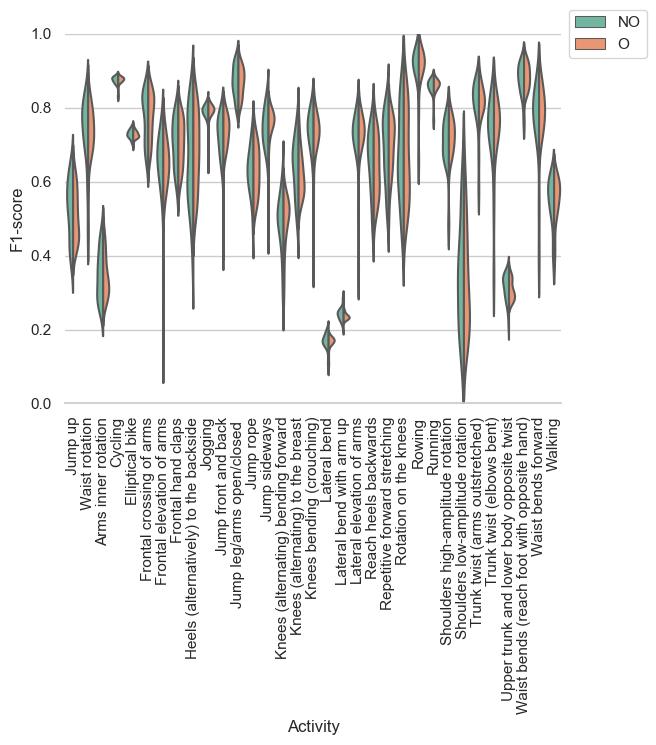
\includegraphics[scale=0.4]{Figures/per_activity_NB_banos_sbj_FS3.png}}
    \subfigure[NCC]{\label{fig:NCC_ds1-activity-exp3}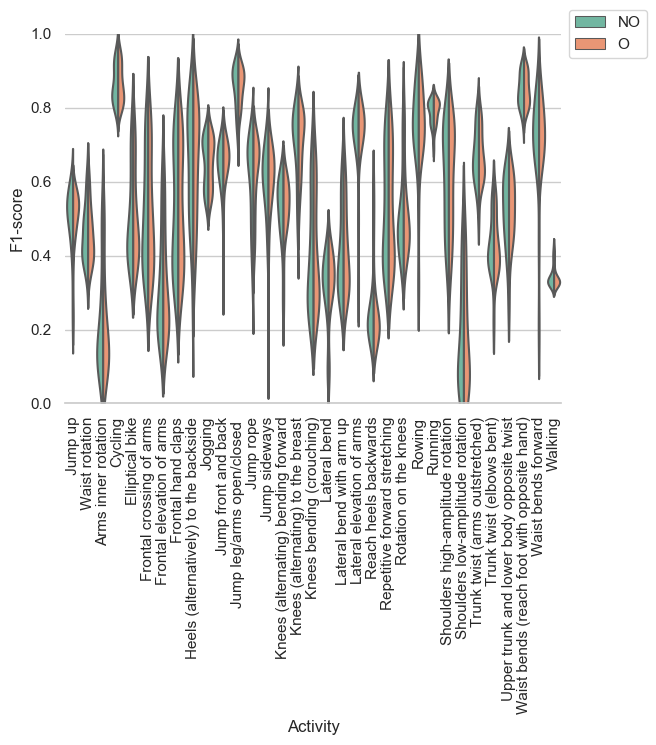
\includegraphics[scale=0.4]{Figures/per_activity_NCC_banos_sbj_FS3.png}}
   
   \caption{Experiment 3 -- Subject-independent CV -- Dataset 1. O and NO stand for overlapping and non-overlapping windowing respectively.}
    \label{fig:exp3_ds1}
    
\end{figure}

\begin{figure}[htp]
  \centering
  \subfigure[DT]{\label{fig:DT_ds2-activity-exp3}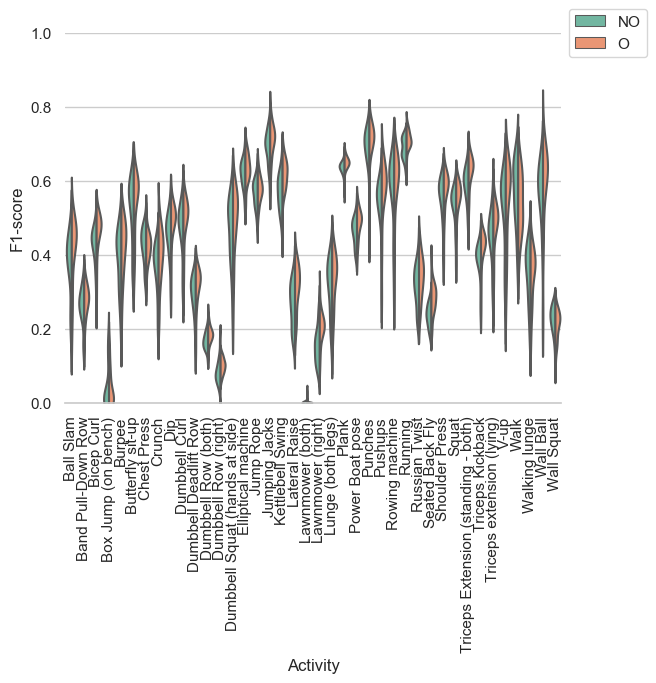
\includegraphics[scale=0.4]{Figures/per_activity_DT_recofit_sbj_FS3.png}}\quad
  \subfigure[KNN]{\label{fig:KNN_ds2-activity-exp3}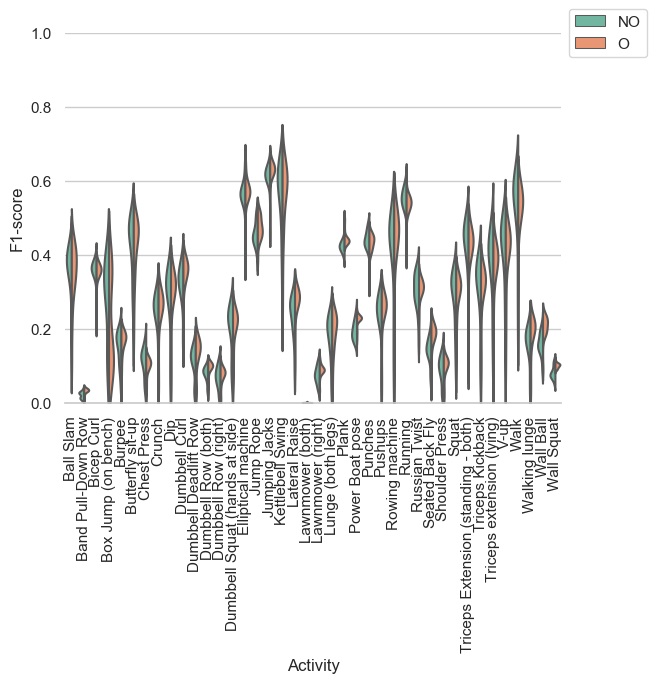
\includegraphics[scale=0.4]{Figures/per_activity_KNN_recofit_sbj_FS3.png}}
  \subfigure[NB]{\label{fig:NB_ds2-activity-exp3}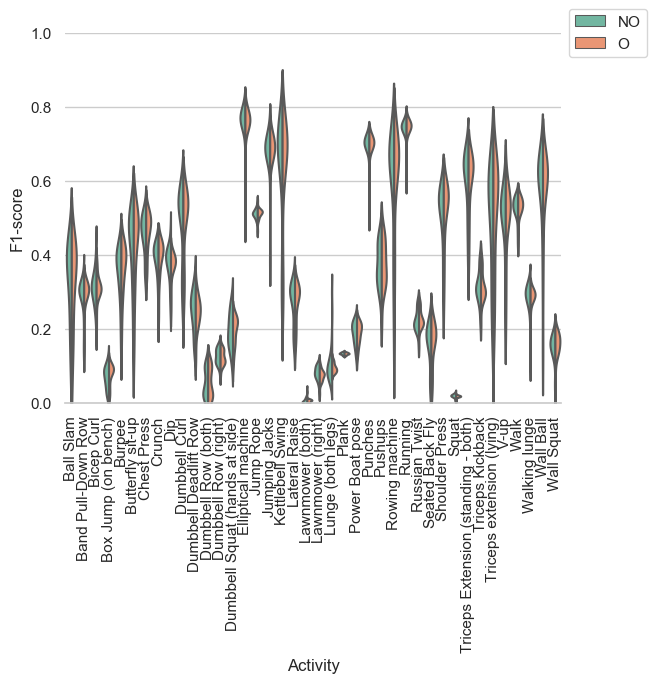
\includegraphics[scale=0.4]{Figures/per_activity_NB_recofit_sbj_FS3.png}}
    \subfigure[NCC]{\label{fig:NCC_ds2-activity-exp3}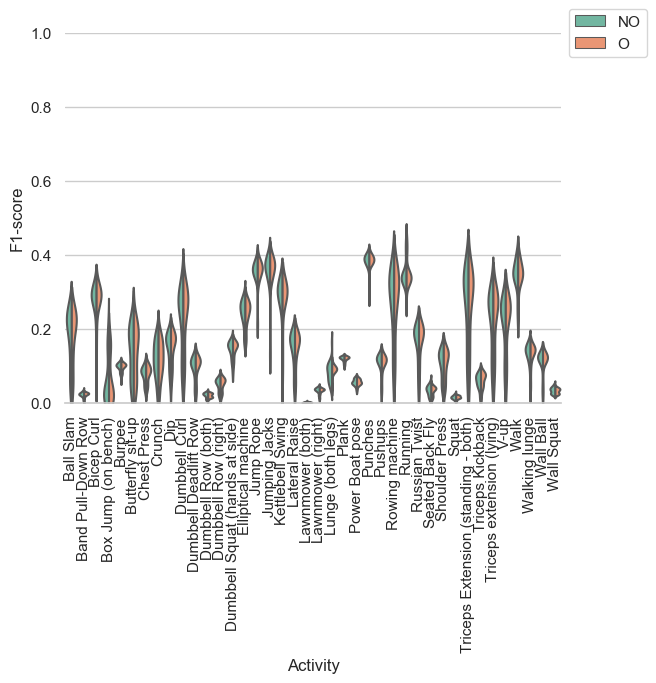
\includegraphics[scale=0.4]{Figures/per_activity_NCC_recofit_sbj_FS3.png}}
   
   \caption{Experiment 3 -- Subject-independent CV -- Dataset 2. O and NO stand for overlapping and non-overlapping windowing respectively.}
    \label{fig:exp3_ds2}
    
\end{figure}

\section{Discussion} \label{sec:discussion}
% Compare the nonoverlapping in sbj dependent and independent CVs
As can be seen by comparing the results of experiment 1 and 2 for non-overlapping windowing, using Subject independent CV instead of 
Subject-dependent CV reduces the F1-score of KNN and DT by 10\% and 11\% on average for Dataset 1 and 2 respectively, which is substantial. It confirms our hypothesis that samples drawn from the 
same subject cannot be considered independent. In an ARP setup, Subject independent CV overestimates the classification performance and should, therefore, be avoided.
% Compare the overlapping in sbj dependent and independent CVs
The detrimental effect of subject-dependent CV is even larger when overlapping time windows are used. In this case, as can be seen by comparing the results of Experiment 1 and 2 for overlapping windowing, Subject-independent CV reduces the F1-score of KNN and DT by 16\% and 21\% on average for Dataset 1 and 2 respectively. This 
further confirms that within-subject dependencies between time windows account for a significant part of the performance measured through 
Subject-dependent CV. Furthermore, for overlapping windows, the performance 
difference between subject-dependent CV and subject independent CV increases with the window 
size. This is consistent with our previous comments, as the amount of 
overlap between overlapping windows, and therefore their correlation, 
also increases with the window size.
% Overlapping windowing is not important once comes with sbj independent
Comparing the results for overlapping and non-overlapping windowing in Figure~\ref{fig:exp1_ds1} and Figure~\ref{fig:exp1_ds2} shows that when using Subject-dependent CV, overlapping windowing can improve the recognition power of the classifiers, which coincides with the general idea that overlapping windowing improves the performance of HAR systems~\cite{janidarmian2017comprehensive,janidarmian2014automated}. 
However, our results confirm that such improvement comes from the 
increasing the correlation among test and train folds due to the underlying 
problems of Subject-dependent CV in HAR systems.      
% Overlapping windowing is not important once comes with sbj independent
In contrast, when using Subject independent CV, the impact of using overlapping
windows is minor to negligible, as can be seen in  
Figure~\ref{fig:exp2_ds1} and Figure~\ref{fig:exp2_ds2}. This is in contradiction with 
the common argument that overlapping windows improve classification
performance by bringing more data to the classifier. However, it also 
confirms our hypothesis that the performance increase coming from 
overlapping windows is, in fact, coming from the extra correlation 
between time windows, when Subject-dependent CV is used.

The results of Experiment 3 show that the impact of overlapping windowing with subject independent CV can be different per activity. In other words, overlapping windowing for some activities such as Trunk Twist and Lateral Raise improves the recognition performances and for others like Repetitive forward stretching and Heels not. However, such improvements and reductions for the most activities are negligible and using this technique in HAR seems to be useless.

Table~\ref{tab:resources} shows the data size and required time for segmentation and training in overlapping and non-overlapping windowing techniques with subject independent CV for two datasets. Segmenting using overlapping windows is almost twice longer than with non-overlaping windows, which is significant. Similarly, training on the data windowed by overlapping windows technique takes 4 times of non-overlapping one. As for storage, the size of segmented data by overlapping sliding windows technique is almost 9 times of data produced by non-overlapping one for both datasets. In spite of such increase in size and computation, this technique does not improve the performance of the classifiers when used with Subject independent CV.

%The resource issues are even worse in active learning


% we use the dataset of two wellknown HAR database which contain different type of activities ranging from ....... .  Having such big distributin of activites help us to be confident about our results.

\begin{table}[]
\begin{tabular}{|c|c|>{\centering}m{1.5cm}|c|>{\centering}m{1.5cm}|c|c|c|}
\hline 
\multirow{2}{*}{Dataset} & \multirow{2}{*}{Raw size (GB)} & \multicolumn{3}{c|}{Nonoverlapping windowing} & \multicolumn{3}{c|}{Overlapping windowing }\tabularnewline
\cline{3-8} \cline{4-8} \cline{5-8} \cline{6-8} \cline{7-8} \cline{8-8} 
 &  & \multicolumn{2}{c|}{Segmentation } & \multirow{2}{1.5cm}{Training time (day)} & \multicolumn{2}{c|}{Segmentation } & \multirow{2}{*}{Training time (day)}\tabularnewline
\cline{1-4} \cline{2-4} \cline{3-4} \cline{4-4} \cline{6-7} \cline{7-7} 
\multicolumn{1}{c}{-} & - & Time (Hour) & Size(GB) &  & Time (Hour) & Size (GB) & \tabularnewline
\hline 
1 & 2.4 & 6.0 & 2.3 & 1.0 & 11.0 & 21 & 4.0\tabularnewline
\hline 
2 & 3.4 & 12.0 & 5.8 & 2.0 & 20.0 & 51 & 8.0\tabularnewline
\hline 
\end{tabular}
        \caption{Overlapping windowing vs. nonoverlapping windowing required resources - Subject independent CV}
        \label{tab:resources}
\end{table}






% comparing the used resources 
%in spite of being dependent on the dataset and activities but we can also say that in this work we compare the impact of overlapping for a wide range of activities 


\section{Conclusion} \label{sec:conclusion}
We conclude that the suggested improvement of HAR systems by using overlapping sliding window in literature is resulted from the underlying problems of subject-dependent CV in this field. Our findings also show that in case of using suitable system evaluation techniques such as subject-independent CV, overlapping sliding window method does not add any values to the HAR systems and the same performance is obtainable using non-overlapping one which is more resource-efficient.

In our future works, we will focus on the extracting more discriminative features to (1) improve the performance of HAR systems evaluated through subject-independent CV (2) enhance the generalizability of HAR systems with a limited number of subjects.  


% We conclude that in contrary to public belief \TG{you should tone this down} about the superiority of overlapping sliding windows technique over non-overlapping sliding windows one in segmentation step of ARP, using that with Subject-independent CV does not improve the activity recognition power of classifiers. In spite of that, this technique needs more resources(CPU, memory, etc) which can be problematic in wearable devices \TG{The conclusion needs to be fleshed out. You should summarize your results and describe future works}.    


\vspace{6pt} 
\authorcontributions{}
Conceptualization, A.D., O.S., T.G. and E.Sh.; methodology, A.D., O.S., T.G. and E.Sh.; software, A.D.; validation, A.D., O.S., T.G. and E.Sh.; formal analysis, A.D., O.S., T.G. and E.Sh.; investigation, A.D., O.S., T.G. and E.Sh.; data curation, A.D., O.S.; writing--original draft preparation, A.D.; writing--review and editing, A.D., O.S., T.G. and E.Sh.; visualization, A.D.; supervision, T.G. and E.Sh.; project administration, E.Sh.; funding acquisition, T.G. and E.Sh.

\funding{}

This work was funded by a Strategic Project Grant from the Natural Sciences and Engineering Research Council of Canada.


\conflictsofinterest{}
The authors declare no conflict of interest.
 \reftitle{References}
\externalbibliography{yes}
\bibliography{refs.bib}
\end{document}

